\begin{recipe}
    [%
        preparationtime = {\unit[5]{min}},
        portion = {\portion{3-4}},
        bakingtime = {\unit[10-15]{min}}
    ]
    {Polish apple crumpets}
    \introduction{%
        This recipe encourages you to explore apples: you need to take an account on their tenderness - the more crisp and firm apple, the thinner the slices!
        How many kinds of apples do you know?
        Granny Smith doesn't count, if I had power, I would erase it!

        PS You don't need muffin rings, in Poland we actually prefer crumpets to be uneven and more oval.
    }

    \ingredients{%
        4 & Apples (big) \\
        1~\nicefrac{1}{2} c. & Milk \\
        1~\nicefrac{1}{2} c. & Flour \\
        3 tbs. & Sugar \\
        1 ts. & Baking powder/soda
    }

    \preparation{%
        \step Mix well all the batter ingredients.

        \step Cut apples into \unit[5-10]{cm} high slices (remove cores).

        \step Dig apple slices in the batter and fry.

        \step Serve with caster sugar or confiture.
    }

    \hint{%
        I prefer to leave apple skin but you can peel it, especially if you use 'allotment apples' or some of the so called 'old kind' such as reinette.
    }

\end{recipe}

\begin{figure}[t]
    \centering
    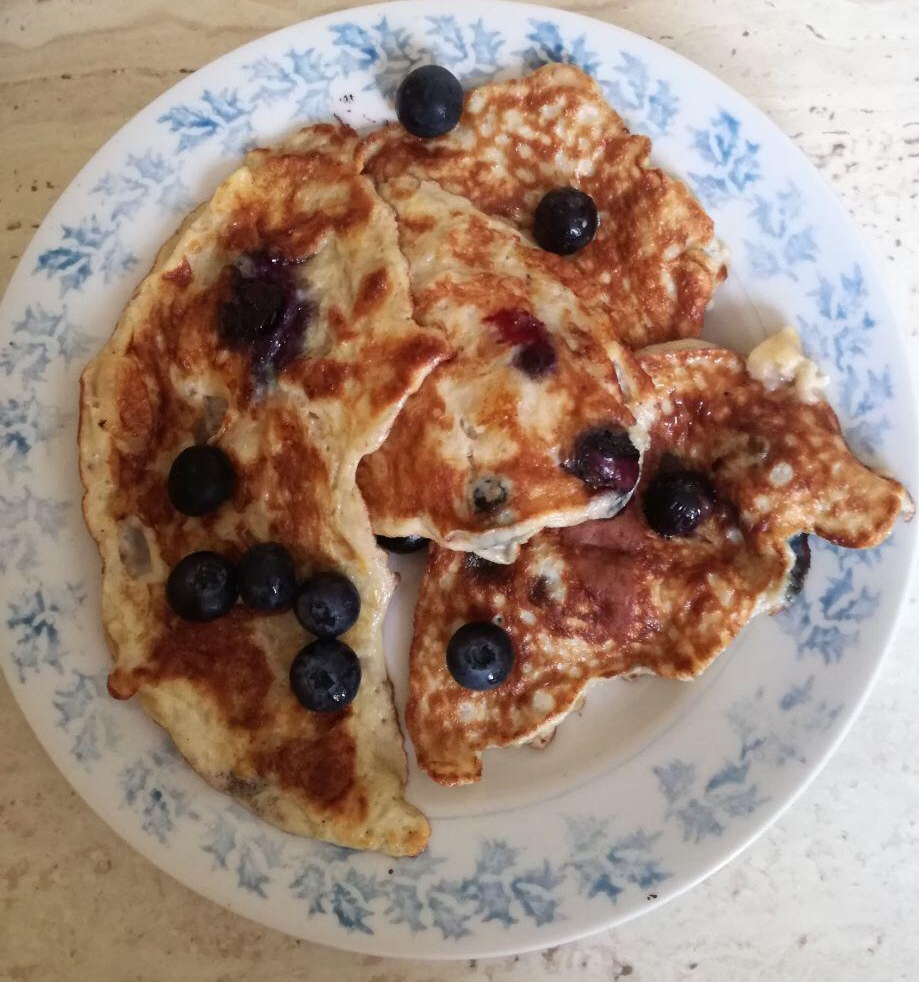
\includegraphics[width=12cm]{pic/crumpets}
\end{figure}
